\documentclass[a4paper]{article}

\usepackage{makeidx}
\usepackage{xcolor}
\usepackage[utf8]{inputenc}
\usepackage[T1]{fontenc}
\usepackage[english]{babel}
\usepackage{mathtools,amssymb,amsmath}
\usepackage{mathrsfs}
\usepackage{mathabx}
\usepackage{yfonts}
\usepackage{geometry}
\usepackage{enumitem}
\usepackage{fancyhdr}
\usepackage{graphicx}
\usepackage{thmbox}
\usepackage{tabularx}
\usepackage{xcolor}
\usepackage{graphicx}
\usepackage{array}
\usepackage{makecell}
\usepackage{multirow}
\usepackage{bbm}
\usepackage{multicol}

\usepackage{tikz}
\usetikzlibrary{calc, quotes}
\usepackage{ifthen}

\geometry{top=3cm,left=2cm,bottom=3cm,right=2cm}

\lhead{}

\renewcommand{\headrulewidth}{0pt}

\newcommand{\N}{\mathbb{N}}
\newcommand{\Z}{\mathbb{Z}}
\newcommand{\D}{\mathbb{D}}
\newcommand{\Q}{\mathbb{Q}}
\newcommand{\R}{\mathbb{R}}
\newcommand{\U}{\mathbb{U}}
\newcommand{\C}{\mathbb{C}}
\newcommand{\K}{\mathbb{K}}
\newcommand{\Pb}{\mathbb{P}}
\newcommand{\Unb}{\mathbbm{1}}
\newcommand{\E}{\mathbb{E}}
\newcommand{\I}{\mathbb{I}}
\newcommand{\T}{\mathbb{T}}
\newcommand{\Sc}{\mathcal{S}}
\newcommand{\Fg}{\mathfrak{F}}
\newcommand{\Ag}{\mathfrak{A}}
\newcommand{\Sg}{\mathfrak{S}}
\newcommand{\Mc}{\mathcal{M}}
\newcommand{\GLc}{\mathcal{GL}}
\newcommand{\SLc}{\mathcal{SL}}
\newcommand{\Bc}{\mathcal{B}}
\newcommand{\Pc}{\mathcal{P}}
\newcommand{\Oc}{\mathcal{O}}
\newcommand{\V}{\mathbb{V}}
\renewcommand{\Im}{\mathrm{Im}}
\newcommand{\Ker}{\mathrm{Ker}}
\renewcommand{\det}{\mathrm{det}}
\newcommand{\argsmin}{\mathrm{argsmin}}
\newcommand{\argsmax}{\mathrm{argsmax}}
\newcommand{\Mat}{\mathrm{Mat}}
\newcommand{\Rac}{\mathrm{Rac}}
\newcommand{\Res}{\mathrm{Res}}
\newcommand{\Var}{\mathrm{Var}}
\newcommand{\cov}{\mathrm{cov}}
\newcommand{\Id}{\mathrm{Id}}
\newcommand{\Supp}{\mathrm{Supp}}
\newcommand{\Cg}{\mathfrak{C}}
\newcommand{\Lg}{\mathfrak{L}}
\newcommand{\ps}[2]{\left\langle#1,#2\right\rangle}
\newcommand{\homeo}{\underset{\text{homeo}}{\clap{$\simeq$}}} % Homeomorph
\newcommand{\nothomeo}{\underset{\text{homeo}}{\clap{$\not\simeq$}}}
\newcommand{\fun}[5]{\begin{array}{cccc}
#1~: & #2 & $\longrightarrow$ & #3 \\
    & #4 & $\longmapsto$ & #5 \end{array}}
\newcommand{\under}[2]{\underbrace{#1}_{\clap{$#2$}}}
\newcommand{\jacobi}[2]{\genfrac{(}{)}{}{1}{#1}{#2}}
\newcommand{\defeq}{\overset{\Delta}{=}}
\newcommand{\Lm}{\preceq_\mathrm{Lm}} % leximin
\newcommand{\Lms}{\precsim_\mathrm{Lm}}

\def\restriction#1#2{\mathchoice
              {\setbox1\hbox{${\displaystyle #1}_{\scriptstyle #2}$}
              \restrictionaux{#1}{#2}}
              {\setbox1\hbox{${\textstyle #1}_{\scriptstyle #2}$}
              \restrictionaux{#1}{#2}}
              {\setbox1\hbox{${\scriptstyle #1}_{\scriptscriptstyle #2}$}
              \restrictionaux{#1}{#2}}
              {\setbox1\hbox{${\scriptscriptstyle #1}_{\scriptscriptstyle #2}$}
              \restrictionaux{#1}{#2}}}
\def\restrictionaux#1#2{{#1\,\smash{\vrule height .8\ht1 depth .85\dp1}}_{\,#2}}


\usepackage[T1]{fontenc}
\usepackage[scaled]{beramono}

\newcommand{\PSS}[1]{\Pb_{SS,#1}}
\newcommand{\PMR}[1]{\Pb_{MR,#1}}
\newcommand{\TE}[1]{\mathfrak{T}_{\mathfrak{E},#1}}
\newcommand{\TM}[1]{\mathfrak{T}_{\mathfrak{M},#1}}
\newcommand{\UnbP}[1]{\Unb_{\Pb_{#1}}}

\newtheorem[style=S, bodystyle=\noindent]{thm}{Theorem}[section]
\newtheorem[style=S, bodystyle=\noindent]{defn}[thm]{Definition}
\newtheorem[style=S, bodystyle=\noindent]{propo}[thm]{Proposition}
\newtheorem[style=S, bodystyle=\noindent]{prop}[thm]{Property}
\newtheorem[style=S, bodystyle=\noindent]{coro}[thm]{Corollary}
\newtheorem[style=S, bodystyle=\noindent]{lem}[thm]{Lemma}
\newtheorem[style=S, headstyle=\bfseries\boldmath Theorem, bodystyle=\noindent]{thm*}{Theorem}
\newtheorem[style=S, headstyle=\bfseries\boldmath Definition, bodystyle=\noindent]{defn*}{Definition}
\newtheorem[style=S, headstyle=\bfseries\boldmath Proposition, bodystyle=\noindent]{propo*}{Proposition}
\newtheorem[style=S, headstyle=\bfseries\boldmath Property, bodystyle=\noindent]{prop*}{Property}
\newtheorem[style=S, headstyle=\bfseries\boldmath Corollary, bodystyle=\noindent]{coro*}{Corollary}
\newtheorem[style=S, headstyle=\bfseries\boldmath Lemma, bodystyle=\noindent]{lem*}{Lemma}

\title{Orders execution.}
\author{}
\date{}
\rhead{}
\allowdisplaybreaks

\begin{document}

\pagestyle{fancy}
\maketitle

\paragraph{}
We are interested in markets with a single order book. Let $(A_i)_{i\in\N^*}$ be the set of agents. We call order a quadruplet of the form $o = (o_A, o_d, o_p, o_q)$ with $o_A \in (A_i)_{i\in\N^*},~o_d \in \{\text{ask},\text{bid}\},~o_p>0$ and $o_q>0$. $\Omega$ denotes the set of orders and $\Omega_n$ denotes the set of parts $\Oc$ from $\Omega$ with n elements such that $\forall o \neq o' \in \Oc,~o_A \neq o'_A$. We also note $w_i$ the wealth of agent \textit{i}, $c_i \geq 0$ its initial cash and $n_i \geq 0$ its initial assets. It is also assumed that agents cannot have negative cash or assets.
\par
If $W$ is a welfare function taking as input the $w_i$, we can define $\tilde W$ taking as input the $(c_i)_{1\leq i\leq n}$, the $(n_i)_{1\leq i\leq n}$ and a sequence of orders $\Oc = (o_1, \ldots, o_n)$ and returning welfare $\tilde W((c_i), n_i)_{1\leq i\leq n}, \Oc)$ after executing the $\Oc$ order sequence on the market initialised with an empty order book and whose agents are initialised with the initial conditions $CI = (c_i, n_i)_{1\leq i\leq n}$. Note $W_{CI} : \Oc \mapsto \tilde W(CI, \Oc)$.


\par
One wonders whether, with $W$ fixed, there is a total order relationship $\preceq$ on the $\Omega$ set of possible orders such that for any finite subset $\Oc = \{o_1, \ldots, o_n\} \in \Omega_n$, for all initial conditions $CI \in \N^{2n}$, the sequence $(o_{\sigma(1)}, \ldots, o_{\sigma(n)})$ such that $o_{\sigma(1)} \preceq \ldots \preceq o_{\sigma(n)}$ maximises the welfare, i.e. : \\
\[W_{CI}(o_{\sigma(1)}, \ldots, o_{\sigma(n)}) = \max_{\tau \in \Sg_n}W_{CI}(o_{\tau(1)}, \ldots, o_{\tau(n)})\]


\par
Note: There is generally no single sequence maximising this welfare. We just require the one sorted by $\preceq$ to  be one of them.

\par We note $\Sg_\Oc$ the set of sequences whose elements are exactly the elements of $\Oc$ and $W_u$ the utilitarian welfare, $W_{\min}$ the min welfare, $W_{\max}$ the max welfare and $W_N$ the Nash welfare. We give ourselves $p_0 \geq 0$: this is the initial price given to the assets when no price has yet been set.

\section{Two-order sequences}


We will show the following (simple) result:
\begin{prop}
If $\Oc \in \Omega_2$, there is a $s \in \Sg_{\mathcal O}$ sequence maximising at once $W_u$, $W_N$, $W_{\min}$ and $W_{\max}$ regardless of the initial conditions.
\end{prop}

\begin{proof}
If both orders have the same direction, or if one is an ask and the other is a bid with $p_\text{ask}$ > $p_\text{bid}$, then no price is set and the result is trivial. \\
In the case where $\mathcal O = \{o_1 = (A_1, \text{ask}, p_a, q_a), o_2 = (A_2, \text{bid}, p_b, q_b)\}$ with $p_b \geq p_a$, let's note $q = \min(q_a,q_b)$. \\
Regardless of the sequence of execution, a price $p\in\{p_a,p_b\}$ will be set and a quantity $q$ will be traded. So we will have $w_1 = (c_1 + qp) + (n_1-q)p = c_1+n_1p$ and $w_2 = (c_2 - qp) + (n_2+q)p = c_2+n_2p$, where $W_u = c_1+c_2+(n_1+n_2)p$, $W_N = (c_1+n_1p)(c_2+n_2p)$, $W_{\min} = \min_i(c_i + n_ip)$ and $W_{\max} = \max_i(c_i + n_ip)$. All these quantities being increasing according to $p$, they are all maximised for the sequence $(o_2, o_1)$ since the fixed price will be $p_b \geq p_a$.
\end{proof}

By the way, we can show the following result:
\begin{prop}
\label{prop1}
If $\mathcal O$ consists of an ask order $o_a$ and a bid order $o_b$, then :
\begin{itemize}
	\item If $p_a \geq p_b$, then the final welfare doesn't depend on the sequence of execution.
	\item If $p_a < p_b$, then $W_u(o_b,o_a) > W_u(o_a,o_b)$ and $W_N(o_b,o_a) > W_N(o_a,o_b)$
	\item If $p_a < p_b$, then $W_{\min}(o_b,o_a) \geq W_{\min}(o_a,o_b)$ with a tie when $n_b = 0$ and $c_b \leq c_a + n_ap_a$.
	\item If $p_a < p_b$, then $W_{\max}(o_b,o_a) \geq W_{\max}(o_a,o_b)$ with equal outcome when $n_b = 0$ and $c_b \geq c_a + n_ap_b$.
\end{itemize}
\end{prop}

\begin{proof}
The first point is trivial and the second point is proven by noticing that $n_a > 0$. \\
The third point is longer to prove: inequality is obvious but the case of equality is not: we have to study when we have $\min(c_a + n_ap_a, c_b + n_bp_a) = \min(c_a + n_ap_b, c_b + n_bp_b)$. As $p_a < p_b$, having $n_b = 0$ is a necessary condition, which brings us back to study when $\min(c_a + n_ap_a, c_b) = \min(c_a + n_ap_b, c_b)$ which is true iff $c_b \leq c_a + n_ap_a$. It is then enough to check that the reciprocal (if $n_b = 0$ and $c_b \leq c_a + n_ap_a$ then we have equality) is true. \\
The fourth point can be treated as the third.
\end{proof}

We notice in the passage that we can't have both the tie case for $W_{\min}$ and the tie case for $W_{\max}$ when $p_a < p_b$.

 \section{Interlude: A useful lemma}

We write down $\argsmax_{x\in X}f(x)$ the set $\{x \in X, f(x) = \max_{y\in X}f(y)\}$.

\begin{lem}
	\label{lem1}
	Let's call it $n \geq 2$. Let $\Oc = \{o_1, \ldots, o_n\} \in \Omega_n$. Let $\Oc'$ and $\Oc''$ be two subsets of $\Oc'$ of zero intersection. Let $W$ be fixed.
	If there exists $CI \in \N^{2n}$ such that , by noting $S = \argsmax_{s \in \Sg_\Oc}W_{CI}(s)$, we have for all $s \in S$ the existence of $o_i\in\Oc'$ and $o_j\in\Oc''$ such that the order $o_i$ appears before $o_j$ in the sequence s, so if $\preceq$ exists, there's $o_i\in\Oc'$ and $o_j\in\Oc'$ such that $o_i \preceq o_j$.
\end{lem}

\begin{proof}
    Under the assumption that $\preceq$ exists, the sequence $s = (o_{\sigma(1)} \preceq \ldots \preceq o_{\sigma(n)})$ maximises $W$ welfare for all initial conditions, so for $CI$ in particular. So $s \in S$. Hypothetically, there is $o_i \in \Oc'$ and $o_j \in \Oc''$ such that $o_i$ appears before $o_j$ in s. So, by definition of $s$, $o_i \preceq o_j$
\end{proof}

From this lemma and the property 1.2 we can deduce that :

\begin{prop}
	\label{prop2}
	If $o_a, o_b \in \Omega^2$ with $o_{a, d} = \text{ask}$, $o_{b, d} = \text{bid}$ and $o_{a, p} < o_{b,p}$, then $o_b \preceq o_a$, if $W = W_u,~W_N,~W_{\min}$ or $W_{\max}$ and if $\preceq$ exists.
\end{prop}


\section{Non-existence of $\preceq$ for the usual welfare}

We'll use these previous results to show that there is no $\preceq$ order on $\Omega$ verifying the desired property.

\subsection{Minimum welfare and welfare of Nash}
~
\begin{thm}
	\label{thm1}
	Either $W = W_{\min}$ or $W_N$. \\
	There's no such thing as a total order $\preceq$ in $\Omega$ such that for any set $\Oc = \{o_1, \ldots, o_n\} \in \Omega_n$, for all initial conditions $CI \in \N^{2n}$, the sequence $(o_{\sigma(1)}, \ldots, o_{\sigma(n)})$ such that $o_{\sigma(1)} \preceq \ldots \preceq o_{\sigma(n)}$ is one of the $\Oc$ sequences maximising welfare $W_{\CI}$.


\end{thm}

\begin{proof}
	~\\
	\textbf{1\up{st} step : It exists $\boldsymbol{\Oc \in \Omega_3}$ made up of two asks orders $\boldsymbol{o_1}$ and $\boldsymbol{o_2}$ and a bid order $\boldsymbol{o_3}$ whose price is higher than those of the orders asks such that nor $\boldsymbol{o_3}$, nor $\boldsymbol{(o_3, o_2, o_1)}$ nor $\boldsymbol{(o_3, o_2, o_1)}$ maximises welfare.} \\
	Let $\Oc = \{o_1 = (A_1, \text{ask}, p_1, q_1) , o_2 = (A_2, \text{ask}, p_2, q_2), o_3 = (A_3, \text{bid}, p_3, q_3)\} \in \Omega_3$ \\ and $CI = (c_i, n_i)_{1\leq i\leq 3} \in \N^6$ such that :

	\begin{multicols}{2}
	\begin{enumerate}
		\item $p_1 < p_3$
		\item $p_2 < p_3$
		\item $q_1 \leq n_1$
		\item $q_2 \leq n_2$
		\item $q_2 < q_3$
		\item $q_3 - q_2 < q_1 < q_3$
		\item $c_3 + n_3p_3 < c_1 + n_1p_3 \\< \min(c_2 + q_2p_2 + n_2p_3 - q_2p_3,\\c_3 - q_2p_2 + q_2p_3 + n_3p_3)$
		\item $q_2(p_3-p_2) < (c_2 + n_2p_3) - (c_3 + n_3p_3)$\\
	\end{enumerate}
	\end{multicols}
	The existence of such $\Oc$ and $CI$ is not self-evident: an example is given in appendix \ref{appendix1}. \\
	The following table shows the cash and the number of assets held by each agent after the execution of different sequences. The last fixed price is, in all cases, $p_3$. The details are given in the appendix
    \ref{appendix2}. \\
	\begin{center}
	\begin{tabular}{|c|c|c|c|c|c|c|}
		\hline
		\multirow{2}{*}{Sequence} & \multicolumn{2}{c|}{$A_1$} & \multicolumn{2}{c|}{$A_2$} & \multicolumn{2}{c|}{$A_3$} \\
		\cline{2-7}
		& cash & assets & cash & assets & cash & assets \\
		\hline
		\multirow{2}{*}{$(o_2, o_3, o_1)$} & \multirow{2}{*}{$c_1 + (q_3-q_2)p_3$} & \multirow{2}{*}{$n_1 - (q_3-q_2)$} & \multirow{2}{*}{$c_2 + q_2p_2$} & \multirow{2}{*}{$n_2-q_2$} & $c_3 - q_2p_2$ & \multirow{2}{*}{$n_3+q_3$} \\
		& & & & &  $-(q_3-q_2)p_3$ & \\
		\hline
		$(o_3,o_1,o_2)$ & $c_1+q_1p_3$ & $n_1-q_1$ & $c_2 + (q_3-q_1)p_3$ & $n_2 - (q_3-q_1)$ & $c_3 - q_3p_3$ & $n_3+q_3$ \\
		\hline
		$(o_3,o_2,o_1)$ & $c_1 + (q_3-q_2)p_3$ & $n_1-(q_3-q_2)$ & $c_2+q_2p_3$ & $n_2-q_2$ & $c_3 - q_3p_3$ & $n_3+q_3$ \\
		\hline
	\end{tabular}
	\end{center}
	So, it just comes that :
	\begin{center}
	\begin{tabular}{|c|c|c|c|}
		\hline
		Sequence & $w_1$ & $w_2$ & $w_3$ \\
		\hline
		$(o_2, o_3, o_1)$ & $c_1 + n_1p_3$ & $c_2+q_2p_2+(n_2-q_2)p_3$ & $c_3+q_2(p_3-p_2)+n_3p_3$ \\
		\hline
		$(o_3,o_1,o_2)$ & \multirow{2}{*}{$c_1+n_1p_3$} & \multirow{2}{*}{$c_2+n_2p_3$} & \multirow{2}{*}{$c_3+n_3p_3$} \\
		\cline{1-1}
		$(o_3,o_2,o_1)$ & & & \\
		\hline
	\end{tabular}
	\end{center}
	Let $(o_3, \cdot, \cdot)$ be the sequences $(o_3,o_1,o_2)$ and $(o_3,o_2,o_1)$. \\
	We conclude that $W_{\min,CI}(o_3, \cdot, \cdot) = \min(c_1+n_1p_3,~c_2+n_2p_3,~c_3+n_3p_3) = c_3+n_3p_3$ according to (7), (8) and (2). \\
	Moreover, $W_{\min, CI}(o_2,o_3,o_1) = \min(c_1 + n_1p_3,~c_2+q_2p_2+(n_2-q_2)p_3,~c_3+q_2(p_3-p_2)+n_3p_3) = c_1 + n_1p_3$ according to (7).
	Finally, (7) also gives that $\boldsymbol{W_{\min,CI}(o_2,o_3,o_1) = c_1 + n_1p_3 > c_3 + n_3p_3 = W_{\min,CI}(o_3, \cdot)}$. We've made it clear what we want for $W_{\min,CI}$. Let's do the same for $W_{\N,CI}$: \\ ~\\
	$W_{N,CI}(o_3, \cdot, \cdot) = (c_1+n_1p_3)(c_2+n_2p_3)(c_3+n_3p_3)$ and \\
	$W_{N,CI}(o_2, o_3, o_1) = (c_1+n_1p_3)(c_2+q_2p_2+(n_2-q_2)p_3)(c_3+q_2(p_3-p_2)+n_3p_3)$, hence \\
	$\begin{array}{rcl}
	\dfrac{W_{N,CI}(o_2, o_3, o_1)}{W_{N,CI}(o_3, \cdot, \cdot)} & = & \dfrac{(c_2+q_2p_2+(n_2-q_2)p_3)(c_3+q_2(p_3-p_2)+n_3p_3)}{(c_2+n_2p_3)(c_3+n_3p_3)} \\
	& = & \ldots \\
	& = & 1 + \dfrac{q_2(p_3-p_2)[(c_2+n_2p_3) - (c_3+n_3p_3) - q_2(p_3-p_2)]}{(c_2+n_2p_3)(c_3+n_3p_3)}
	\end{array}$ \\
	with $q_2\underbrace{(p_3-p_2)}_{> 0 \text{ as per (2)}}\underbrace{[(c_2+n_2p_3) - (c_3+n_3p_3) - q_2(p_3-p_2)]}_{>0 \text{ as per (8)}} > 0$. \\
	So $\boldsymbol{W_{N, CI}(o_2,o_3,o_1) > W_{N,CI}(o_3, \cdot, \cdot)}$.\\~\\
	\textbf{2\up{nd} step : Conclusion} \\
	If by any chance there was an order relationship $\preceq_{\min}$ (resp. $\preceq_{\N}$) on $\Omega$ such that for any set $\Oc' = \{o'_1, \ldots, o'_n\} \in \Omega_n$, for all initial conditions $CI' \in \N^{2n}$, the sequence $(o'_{\sigma(1)}, \ldots, o'_{\sigma(n)})$ such that $o'_{\sigma(1)} \preceq \ldots \preceq o'_{\sigma(n)}$ is one of the $\Oc'$ sequences maximising welfare $W_{\min,CI'}$, so: \\
	As $o_3$ is a bid and as $o_1, o_2$ are asks such that $p_1 < p_3$ (1) and $p_2 < p_3$ (2), then from the property \ref{prop2} comes the fact that $o_3 \preceq_{\min} o_1$, $o_3 \preceq_{\min} o_2$, $o_3 \preceq_N o_1$ and $o_3 \preceq_N o_2$. These inequalities are even strict because $o_1, o_2$ and $o_3$ are distinct. $o_3$ is therefore both the minimum of $\Oc$ for $\preceq_{\min}$ and for $\preceq_N$. The $\preceq_{\min}$ and $\preceq_N$ sequences of $\Oc$ ordered respectively according to $\preceq_{\min}$ and $\preceq_N$ begin both with $o_3$ i.e. are of the form $(o_3, \cdot)$. By hypothesis, $s_{\min}$ (resp. $s_{N}$) is thus a point at which $W_{\min, CI}$ (resp. $W_{N, CI}$) reaches its maximum, which contradicts the results of the first step.
\end{proof}

\subsection{Maximum welfare}
~
\begin{thm}
	\label{thm2}
	There's no such thing as a total order of $\preceq$ on $\Omega$ such that for any set $\Oc = \{o_1, \ldots, o_n\} \in \Omega_n$, for all initial conditions $CI \in \N^{2n}$, the sequence $(o_{\sigma(1)}, \ldots, o_{\sigma(n)})$ such that $o_{\sigma(1)} \preceq \ldots \preceq o_{\sigma(n)}$ is one of the $\Oc$ sequences maximising the welfare $W_{\max, CI}$.
\end{thm}

\begin{proof}
	The evidence is identical in all respects to the evidence for $W_{\min}$: the second step is identical, so we will just specify the first step. \\
	\textbf{1\up{st} step: There is $\boldsymbol{\Oc \in \Omega_3}$ made up of two orders asks $\boldsymbol{o_1}$ and $\boldsymbol{o_2}$ and a bid order $\boldsymbol{o_3}$ whose price is higher than those of the orders asks such that nor $\boldsymbol{o_3}$, nor $\boldsymbol{(o_3, o_2, o_1)}$ nor $\boldsymbol{(o_3, o_2, o_1)}$ maximises welfare.} \\
	Let $\Oc = \{o_1 = (A_1, \text{ask}, p_1, q_1) , o_2 = (A_2, \text{ask}, p_2, q_2), o_3 = (A_3, \text{bid}, p_3, q_3)\} \in \Omega_3$ \\ and let $CI = (c_i, n_i)_{1\leq i\leq 3} \in \N^6$ such that :
	\begin{multicols}{2}
	\begin{enumerate}
		\item $p_1 < p_3$
		\item $p_2 < p_3$
		\item $q_1 \leq n_1$
		\item $q_2 \leq n_2$\\
		\item $q_1 < q_3 < q_2$
		\item $q_3p_3 < c_3$
		\item $\max(c_1+q_1p_1+(n_1-q_1)p_3,~c_2+n_2p_3) \\ < c_3+q_1(p_3-p_1)+n_3p_3$
		\item $\max(c_1+n_1p_3,~c_2+n_2p_3) < c_3+n_3p_3$
	\end{enumerate}
	\end{multicols}
	An example is provided in Appendix 3.
	The following table shows the cash and the number of assets held by each agent after the execution of different sequences. The last fixed price is, in all cases, $p_3$. The details are given in the appendix \ref{appendix4}. \\
	\begin{center}
	\begin{tabular}{|c|c|c|c|c|c|c|}
		\hline
		\multirow{2}{*}{Sequence} & \multicolumn{2}{c|}{$A_1$} & \multicolumn{2}{c|}{$A_2$} & \multicolumn{2}{c|}{$A_3$} \\
		\cline{2-7}
		& cash & assets & cash & assets & cash & assets \\
		\hline
		\multirow{2}{*}{$(o_1, o_3, o_2)$} & \multirow{2}{*}{$c_1 + q_1p_1$} & \multirow{2}{*}{$n_1-q_1$} & \multirow{2}{*}{$c_2 + (q_3-q_1)p_3$} & \multirow{2}{*}{$n_2-(q_3-q_1)$} & $c_1 - q_1p_1$ & \multirow{2}{*}{$n_3+q_3$} \\
		& & & & &  $-(q_3-q_1)p_3$ & \\
		\hline
		$(o_3,o_1,o_2)$ & $c_1+q_1p_3$ & $n_1-q_1$ & $c_2 + (q_3-q_1)p_3$ & $n_2 - (q_3-q_1)$ & $c_3 - q_3p_3$ & $n_3+q_3$ \\
		\hline
		$(o_3,o_2,o_1)$ & $c_1$ & $n_1$ & $c_2+q_3p_3$ & $n_2-q_3$ & $c_3-q_3p_3$ & $n_3+q_3$ \\
		\hline
	\end{tabular}
	\end{center}
	So, it turns out that :
	\begin{center}
	\begin{tabular}{|c|c|c|c|}
		\hline
		Sequence & $w_1$ & $w_2$ & $w_3$ \\
		\hline
		$(o_1, o_3, o_2)$ & $c_1 + q_1p_1 + (n_1-q_1)p_3$ & $c_2+n_2p_3$ & $c_3+q_1(p_3-p_1)+n_3p_3$ \\
		\hline
		$(o_3,o_1,o_2)$ & \multirow{2}{*}{$c_1+n_1p_3$} & \multirow{2}{*}{$c_2+n_2p_3$} & \multirow{2}{*}{$c_3+n_3p_3$} \\
		\cline{1-1}
		$(o_3,o_2,o_1)$ & & & \\
		\hline
	\end{tabular}
	\end{center}
	Denote as $(o_3, \cdot, \cdot)$ the sequences $(o_3,o_1,o_2)$ and $(o_3,o_2,o_1)$. \\
	We have $W_{\max,CI}(o_3, \cdot, \cdot) = \max(c_1+n_1p_3,~c_2+n_2p_3,~c_3+n_3p_3) = c_3+n_3p_3$ according to (8). \\
	And $W_{\max,CI}(o_1, o_3, o_2) = \max(c_1 + q_1p_1 + (n_1-q_1)p_3,~c_2+n_2p_3,~c_3+q_1(p_3-p_1)+n_3p_3) = c_3+q_1(p_3-p_1)+n_3p_3$ according to (7), \\
    hence $\boldsymbol{W_{\max,CI}(o_3, \cdot, \cdot) = c_3+n_3p_3 < c_3+q_1(p_3-p_1)+n_3p_3 = W_{\max,CI}(o_1, o_3, o_2)}$ according to (1).
\end{proof}

\subsection{Utility welfare}

Note in this part the initial conditions $CI = (c_i(0), n_i(0))_{1\leq i\leq n}$. We call $t+1$ the time instant at which the first order is placed or the first price is set from instant $t$.

\begin{lem}
	Let $CI$ be fixed. \\
	There is $C\geq $0 and $N\geq $0 such that $\forall \Oc = \{o_1, \ldots, o_n\}\in \Omega_n, \forall m \leq n$, $W_{u, CI}(o_1), \ldots, o_m) = C + Np_m$ where $p_m$ is the last order set after execution of the sequence $(o_1, \ldots, o_m)$.
\end{lem}

\begin{proof}
	Let $t \geq 0$.\\
	If the time $t+1$ was fixed by a placed order, we trivially have $\sum_{1\leq i\leq n}c_i(t+1) = \sum_{1\leq i\leq n}c_i(t)$ and $\sum_{1\leq i\leq n}n_i(t+1) = \sum_{1\leq i\leq n}n_i(t)$. \\
	If $t+1$ was fixed by a price that was fixed, note $A_i$ the agent from which the ask order originated, $A_j$ the agent from which the bid originated, $q$ the quantity traded and $p$ the fixed price. We have $\forall k \not\in \{i,j\}, c_k(t+1) = c_k(t)$ and $n_k(t+1) = n_k(t)$ and : \\
	$c_i(t+1) = c_i(t) + qp$, $n_i(t+1) = n_i(t) - q$, $c_j(t+1) = c_j(t) - qp$ and $n_j(t+1) = n_j(t) + q$. \\
	So $\sum_{1\leq i\leq n}c_i(t+1) = \sum_{1\leq i\leq n}c_i(t)$ and $\sum_{1\leq i\leq n}n_i(t+1) = \sum_{1\leq i\leq n}n_i(t)$ in all cases: $\sum_ic_i$ and $\sum_in_i$ are constant. They are noted as $C$ and $N$ respectively.
	Then $W_{u,CI}(t) = \sum_iw_i(t) = \sum_i c_i(t) + n_i(t)p = C + Np$ with $p$ the last fixed price.
\end{proof}

In fact, it can be shown that there are no counter-examples with 3 orders, but there are counter-examples with 4 orders.
\section{Leximin welfare}

\subsection{Formalism}
~
\begin{defn}[Pre-order total leximin]
    Be $n\in\N^*$ and $x,y \in \R^n$. We define the total pre-order leximin $\Lm$ by $x \Lm y$ iff, noting $\sigma, \tau \in \Sg_n$ of the permutations such that $x_{\sigma(1)} \leq \ldots \leq x_{\sigma(n)}$ and $y_{\tau(1)} \leq \ldots \leq y_{\tau(n)}$, there is $k \in [\![1,n+1]\!]$ such that $\forall i < k, x_{\sigma(i)} = y_{\tau(i)}$ and, if $k \leq n$, $x_{\sigma(k)} < y_{\tau(k)}$. \\
	Informally, $x$ is smaller than $y$ when the sequence of x coordinates sorted in ascending order is lexicographically smaller than the sequence of y coordinates sorted the same way in ascending order.
\end{defn}

\par
We then divide $\R^n$ by the equivalence relation $\sim$ defined by $x\sim y$ when $x \Lm y$ and $y \Lm x$ (i.e. when the coordinates of x are a permutation of the coordinates of y). The relation $\Lms$ on $\R^n/\sim$ defined by $X\Lms Y$ when $\forall x \in X,\forall y \in Y, x\Lm y$ is then a relation of total order \footnote{Bourbaki, \'Eléments de mathématique : Théorie des ensembles, Paris, Masson, 1998, ch III, \S 1, n^{o}2, p3} on $\R^n/\sim$. For a finite part $P$ of $\R^n$, we then define $\max_{\Lms}P$ as being equal to the intersection between $P$ and the maximum of $\{\bar x, x \in P\}$ for $\Lms$, where $\bar x$ designates the equivalence class of $x$ by $\sim$.

\par
One wonders whether, by calling welfare leximin $W$ the identity function defined on the union of $R^n$ with $n\in\N^*$, there is a total order $\preceq$ on $\Omega$ such that for any $n$, for any $\Oc = \{o_1,\ldots,o_n\}\in\Omega_n$, for all initial conditions $CI\in\N^{2n}$, we have $W_{\CI}(o_{\sigma(1)},\ldots,o_{\sigma(n)}) \in \max_{\Lms, \tau \Sg_n}W_{\CI}(o_{\tau(1)}, \ldots, o_{\tau(n)})$ with $\sigma \in \Sg_n$ such that $o_{\sigma(1)} \preceq \ldots \preceq o_{\sigma(n)}$.

The answer is no: just take the counter-example of $W_{\min}$ (and the property \ref{prop1} remains true).

\newpage
\appendix

\section{Details of the proof of the theorem \ref{thm1}}

\subsection{Example of $\Oc$ and $CI$ sets testing assumptions}
\label{appendix1}
\begin{center}
$\begin{array}{|c|c|c|c|c|}
	\hline
	i & p_i & q_i & c_i & n_i \\
	\hline
	1 & 1463 & 3 & 20932 & 4 \\
	\hline
	2 & 1248 & 4 & 45856 & 24 \\
	\hline
	3 & 5528 & 6 & 12339 & 5 \\
	\hline
\end{array}$
\end{center}

\subsection{Proof of the values obtained for cash and assets after the execution of different sequences}
\label{appendix2}

\par
An order book is represented as follows:
\begin{center}
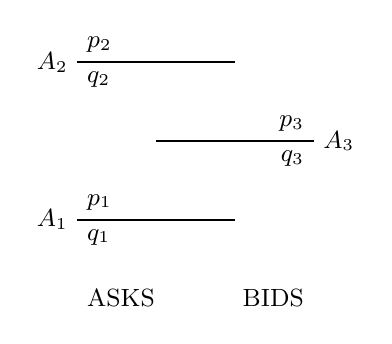
\begin{tikzpicture}
\node [right] at (0,0) {\small ASKS};
\node [left] at (3,0) {\small BIDS};
\draw [thick] (0,1) --(2,1);
\node [above right] at (0,1) {\small $p_1$};
\node [below right] at (0,1) {\small $q_1$};
\node [left] at (0,1) {\small $A_1$};
\draw [thick] (1,2) --(3,2);
\node [above left] at (3,2) {\small $p_3$};
\node [below left] at (3,2) {\small $q_3$};
\node [right] at (3,2) {\small $A_3$};
\draw [thick] (0,3) --(2,3);
\node [above right] at (0,3) {\small $p_2$};
\node [below right] at (0,3) {\small $q_2$};
\node [left] at (0,3) {\small $A_2$};
\end{tikzpicture}
\end{center}
where, in this example, $A_i$ is an agent having placed an order at price $p_i$ for a quantity $q_i$. Orders 1 and 2 are asks, order 3 is a bid, and the vertical scale is the price scale: $p_1 < p_3 < p_2$.

\subsubsection{Sequence $(o_2,o_3,o_1)$}

~\begin{center}
\begin{tabular}{c|c|c}
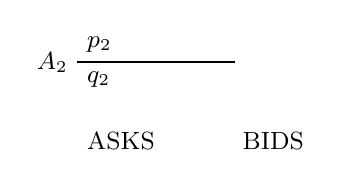
\begin{tikzpicture}
\node [right] at (0,0) {\small ASKS};
\node [left] at (3,0) {\small BIDS};
\draw [thick] (0,1) --(2,1);
\node [above right] at (0,1) {\small $p_2$};
\node [below right] at (0,1) {\small $q_2$};
\node [left] at (0,1) {\small $A_2$};
\end{tikzpicture}
&
\begin{tikzpicture}
\node [right] at (0,0) {\small ASKS};
\node [left] at (3,0) {\small BIDS};
\draw [thick] (0,1) --(2,1);
\node [above right] at (0,1) {\small $p_2$};
\node [below right] at (0,1) {\small $q_2$};
\node [left] at (0,1) {\small $A_2$};
\draw [thick] (1,3) --(3,3);
\node [above left] at (3,3) {\small $p_3$};
\node [below left] at (3,3) {\small $q_3$};
\node [right] at (3,3) {\small $A_3$};
\end{tikzpicture}
&
\begin{tikzpicture}
\node [right] at (0,0) {\small ASKS};
\node [left] at (3,0) {\small BIDS};
\draw [thick] (1,3) --(3,3);
\node [above left] at (3,3) {\small $p_3$};
\node [below left] at (3,3) {\small $q_3-q_2$};
\node [right] at (3,3) {\small $A_3$};
\end{tikzpicture}
\\
Addition of $o_2$ & Addition of $o_3$ & Match between $o_2$ and $o_3$
\end{tabular} \\ \vspace{1cm}
\begin{tabular}{c|c}
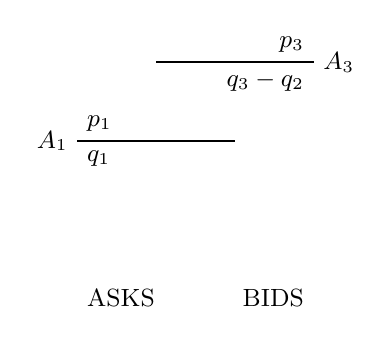
\begin{tikzpicture}
\node [right] at (0,0) {\small ASKS};
\node [left] at (3,0) {\small BIDS};
\draw [thick] (0,2) --(2,2);
\node [above right] at (0,2) {\small $p_1$};
\node [below right] at (0,2) {\small $q_1$};
\node [left] at (0,2) {\small $A_1$};
\draw [thick] (1,3) --(3,3);
\node [above left] at (3,3) {\small $p_3$};
\node [below left] at (3,3) {\small $q_3-q_2$};
\node [right] at (3,3) {\small $A_3$};
\end{tikzpicture}
&
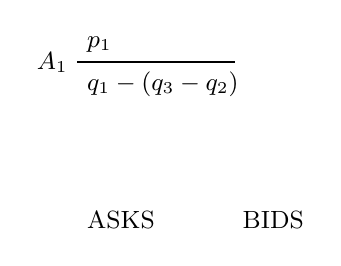
\begin{tikzpicture}
\node [right] at (0,0) {\small ASKS};
\node [left] at (3,0) {\small BIDS};
\draw [thick] (0,2) --(2,2);
\node [above right] at (0,2) {\small $p_1$};
\node [below right] at (0,2) {\small $q_1 - (q_3-q_2)$};
\node [left] at (0,2) {\small $A_1$};
\end{tikzpicture}
\\
Addition of $o_1$ & Match between $o_1$ and $o_3$.
\end{tabular}
\end{center}~
\newpage
\subsubsection{Sequence $(o_3,o_1,o_2)$}

~\begin{center}
\begin{tabular}{c|c|c}
\begin{tikzpicture}
\node [right] at (0,0) {\small ASKS};
\node [left] at (3,0) {\small BIDS};
\draw [thick] (1,3) --(3,3);
\node [above left] at (3,3) {\small $p_3$};
\node [below left] at (3,3) {\small $q_3$};
\node [right] at (3,3) {\small $A_3$};
\end{tikzpicture}
&
\begin{tikzpicture}
\node [right] at (0,0) {\small ASKS};
\node [left] at (3,0) {\small BIDS};
\draw [thick] (0,2) --(2,2);
\node [above right] at (0,2) {\small $p_1$};
\node [below right] at (0,2) {\small $q_1$};
\node [left] at (0,2) {\small $A_1$};
\draw [thick] (1,3) --(3,3);
\node [above left] at (3,3) {\small $p_3$};
\node [below left] at (3,3) {\small $q_3$};
\node [right] at (3,3) {\small $A_3$};
\end{tikzpicture}
&
\begin{tikzpicture}
\node [right] at (0,0) {\small ASKS};
\node [left] at (3,0) {\small BIDS};
\draw [thick] (1,3) --(3,3);
\node [above left] at (3,3) {\small $p_3$};
\node [below left] at (3,3) {\small $q_3-q_1$};
\node [right] at (3,3) {\small $A_3$};
\end{tikzpicture}
\\
Addition of $o_3$ & Addition of $o_1$ & Match between $o_1$ and $o_3$
\end{tabular} \\ \vspace{1cm}
\begin{tabular}{c|c}
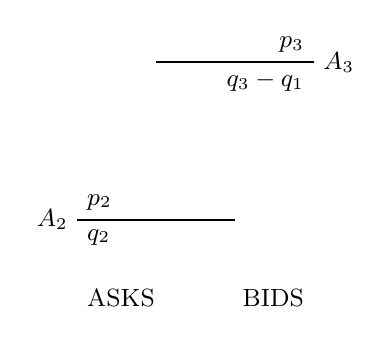
\begin{tikzpicture}
\node [right] at (0,0) {\small ASKS};
\node [left] at (3,0) {\small BIDS};
\draw [thick] (0,1) --(2,1);
\node [above right] at (0,1) {\small $p_2$};
\node [below right] at (0,1) {\small $q_2$};
\node [left] at (0,1) {\small $A_2$};
\draw [thick] (1,3) --(3,3);
\node [above left] at (3,3) {\small $p_3$};
\node [below left] at (3,3) {\small $q_3-q_1$};
\node [right] at (3,3) {\small $A_3$};
\end{tikzpicture}
&
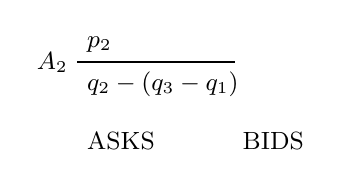
\begin{tikzpicture}
\node [right] at (0,0) {\small ASKS};
\node [left] at (3,0) {\small BIDS};
\draw [thick] (0,1) --(2,1);
\node [above right] at (0,1) {\small $p_2$};
\node [below right] at (0,1) {\small $q_2-(q_3-q_1)$};
\node [left] at (0,1) {\small $A_2$};
\end{tikzpicture}
\\
Addition of $o_2$ & Match between $o_2$ and $o_3$.
\end{tabular}
\end{center}~

\subsubsection{Sequence $(o_3,o_2,o_1)$}

~\begin{center}
\begin{tabular}{c|c|c}
\begin{tikzpicture}
\node [right] at (0,0) {\small ASKS};
\node [left] at (3,0) {\small BIDS};
\draw [thick] (1,3) --(3,3);
\node [above left] at (3,3) {\small $p_3$};
\node [below left] at (3,3) {\small $q_3$};
\node [right] at (3,3) {\small $A_3$};
\end{tikzpicture}
&
\begin{tikzpicture}
\node [right] at (0,0) {\small ASKS};
\node [left] at (3,0) {\small BIDS};
\draw [thick] (0,1) --(2,1);
\node [above right] at (0,1) {\small $p_2$};
\node [below right] at (0,1) {\small $q_2$};
\node [left] at (0,1) {\small $A_2$};
\draw [thick] (1,3) --(3,3);
\node [above left] at (3,3) {\small $p_3$};
\node [below left] at (3,3) {\small $q_3$};
\node [right] at (3,3) {\small $A_3$};
\end{tikzpicture}
&
\begin{tikzpicture}
\node [right] at (0,0) {\small ASKS};
\node [left] at (3,0) {\small BIDS};
\draw [thick] (1,3) --(3,3);
\node [above left] at (3,3) {\small $p_3$};
\node [below left] at (3,3) {\small $q_3-q_2$};
\node [right] at (3,3) {\small $A_3$};
\end{tikzpicture}
\\
Addition of $o_3$ & Addition of $o_2$ & Match between $o_2$ and $o_3$

\end{tabular} \\ \vspace{1cm}
\begin{tabular}{c|c}
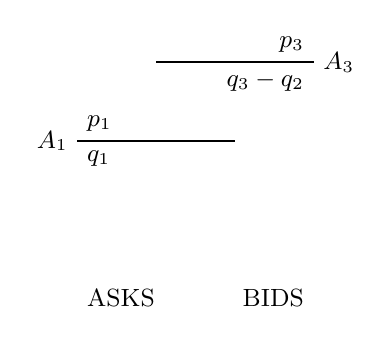
\begin{tikzpicture}
\node [right] at (0,0) {\small ASKS};
\node [left] at (3,0) {\small BIDS};
\draw [thick] (0,2) --(2,2);
\node [above right] at (0,2) {\small $p_1$};
\node [below right] at (0,2) {\small $q_1$};
\node [left] at (0,2) {\small $A_1$};
\draw [thick] (1,3) --(3,3);
\node [above left] at (3,3) {\small $p_3$};
\node [below left] at (3,3) {\small $q_3-q_2$};
\node [right] at (3,3) {\small $A_3$};
\end{tikzpicture}
&
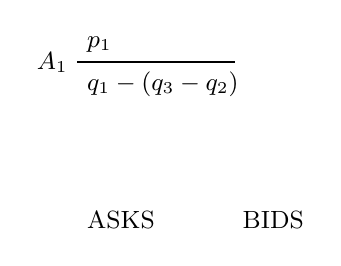
\begin{tikzpicture}
\node [right] at (0,0) {\small ASKS};
\node [left] at (3,0) {\small BIDS};
\draw [thick] (0,2) --(2,2);
\node [above right] at (0,2) {\small $p_1$};
\node [below right] at (0,2) {\small $q_1-(q_3-q_2)$};
\node [left] at (0,2) {\small $A_1$};
\end{tikzpicture}
\\
Addition of $o_1$ & Match between $o_1$ and $o_3$.
\end{tabular}
\end{center}~

\section{Details of the proof of the theorem \ref{thm2}}

\subsection{Example of $\Oc$ and $CI$ verifying the hypotheses}
\label{appendix3}
\begin{center}
$\begin{array}{|c|c|c|c|c|}
	\hline
	i & p_i & q_i & c_i & n_i \\
	\hline
	1 & 1166 & 1 & 23500 & 11 \\
	\hline
	2 & 1002 & 13 & 14969 & 15 \\
	\hline
	3 & 2048 & 11 & 32763 & 24 \\
	\hline
\end{array}$
\end{center}

\subsection{Proof of the values obtained for cash and assets after the execution of different sequences}
\label{appendix4}
~
\subsubsection{Sequence $(o_1,o_3,o_2)$}

~\begin{center}
\begin{tabular}{c|c|c}
\begin{tikzpicture}
\node [right] at (0,0) {\small ASKS};
\node [left] at (3,0) {\small BIDS};
\draw [thick] (0,2) --(2,2);
\node [above right] at (0,2) {\small $p_1$};
\node [below right] at (0,2) {\small $q_1$};
\node [left] at (0,2) {\small $A_1$};
\end{tikzpicture}
&
\begin{tikzpicture}
\node [right] at (0,0) {\small ASKS};
\node [left] at (3,0) {\small BIDS};
\draw [thick] (0,2) --(2,2);
\node [above right] at (0,2) {\small $p_1$};
\node [below right] at (0,2) {\small $q_1$};
\node [left] at (0,2) {\small $A_1$};
\draw [thick] (1,3) --(3,3);
\node [above left] at (3,3) {\small $p_3$};
\node [below left] at (3,3) {\small $q_3$};
\node [right] at (3,3) {\small $A_3$};
\end{tikzpicture}
&
\begin{tikzpicture}
\node [right] at (0,0) {\small ASKS};
\node [left] at (3,0) {\small BIDS};
\draw [thick] (1,3) --(3,3);
\node [above left] at (3,3) {\small $p_3$};
\node [below left] at (3,3) {\small $q_3-q_1$};
\node [right] at (3,3) {\small $A_3$};
\end{tikzpicture}
\\
Addition of $o_1$ & Addition of $o_3$ & Match between $o_1$ and $o_3$
\end{tabular} \\ \vspace{1cm}
\begin{tabular}{c|c}
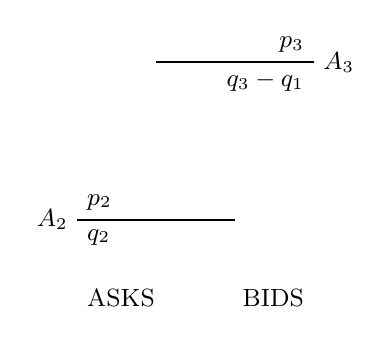
\begin{tikzpicture}
\node [right] at (0,0) {\small ASKS};
\node [left] at (3,0) {\small BIDS};
\draw [thick] (0,1) --(2,1);
\node [above right] at (0,1) {\small $p_2$};
\node [below right] at (0,1) {\small $q_2$};
\node [left] at (0,1) {\small $A_2$};
\draw [thick] (1,3) --(3,3);
\node [above left] at (3,3) {\small $p_3$};
\node [below left] at (3,3) {\small $q_3-q_1$};
\node [right] at (3,3) {\small $A_3$};
\end{tikzpicture}
&
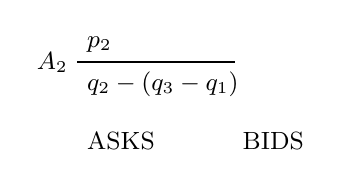
\begin{tikzpicture}
\node [right] at (0,0) {\small ASKS};
\node [left] at (3,0) {\small BIDS};
\draw [thick] (0,1) --(2,1);
\node [above right] at (0,1) {\small $p_2$};
\node [below right] at (0,1) {\small $q_2-(q_3-q_1)$};
\node [left] at (0,1) {\small $A_2$};
\end{tikzpicture}
\\
Addition of $o_2$ & Match between $o_2$ and $o_3$.
\end{tabular}
\end{center}~
\newpage
\subsubsection{Sequence $(o_3,o_1,o_2)$}

~\begin{center}
\begin{tabular}{c|c|c}
\begin{tikzpicture}
\node [right] at (0,0) {\small ASKS};
\node [left] at (3,0) {\small BIDS};
\draw [thick] (1,3) --(3,3);
\node [above left] at (3,3) {\small $p_3$};
\node [below left] at (3,3) {\small $q_3$};
\node [right] at (3,3) {\small $A_3$};
\end{tikzpicture}
&
\begin{tikzpicture}
\node [right] at (0,0) {\small ASKS};
\node [left] at (3,0) {\small BIDS};
\draw [thick] (0,2) --(2,2);
\node [above right] at (0,2) {\small $p_1$};
\node [below right] at (0,2) {\small $q_1$};
\node [left] at (0,2) {\small $A_1$};
\draw [thick] (1,3) --(3,3);
\node [above left] at (3,3) {\small $p_3$};
\node [below left] at (3,3) {\small $q_3$};
\node [right] at (3,3) {\small $A_3$};
\end{tikzpicture}
&
\begin{tikzpicture}
\node [right] at (0,0) {\small ASKS};
\node [left] at (3,0) {\small BIDS};
\draw [thick] (1,3) --(3,3);
\node [above left] at (3,3) {\small $p_3$};
\node [below left] at (3,3) {\small $q_3-q_1$};
\node [right] at (3,3) {\small $A_3$};
\end{tikzpicture}
\\
Addition of $o_3$ & Addition of $o_1$ & Match between $o_1$ and $o_3$
\end{tabular} \\ \vspace{1cm}
\begin{tabular}{c|c}
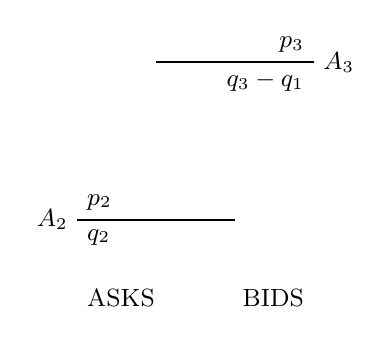
\begin{tikzpicture}
\node [right] at (0,0) {\small ASKS};
\node [left] at (3,0) {\small BIDS};
\draw [thick] (0,1) --(2,1);
\node [above right] at (0,1) {\small $p_2$};
\node [below right] at (0,1) {\small $q_2$};
\node [left] at (0,1) {\small $A_2$};
\draw [thick] (1,3) --(3,3);
\node [above left] at (3,3) {\small $p_3$};
\node [below left] at (3,3) {\small $q_3-q_1$};
\node [right] at (3,3) {\small $A_3$};
\end{tikzpicture}
&
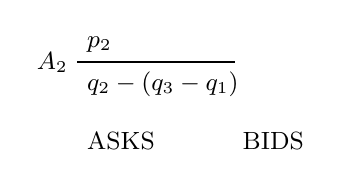
\begin{tikzpicture}
\node [right] at (0,0) {\small ASKS};
\node [left] at (3,0) {\small BIDS};
\draw [thick] (0,1) --(2,1);
\node [above right] at (0,1) {\small $p_2$};
\node [below right] at (0,1) {\small $q_2-(q_3-q_1)$};
\node [left] at (0,1) {\small $A_2$};
\end{tikzpicture}
\\
Addition of $o_2$ & Match between $o_2$ and $o_3$.
\end{tabular}
\end{center}~

\subsubsection{Sequence $(o_3,o_2,o_1)$}

~\begin{center}
\begin{tabular}{c|c|c|c}
\begin{tikzpicture}
\node [right] at (0,0) {\small ASKS};
\node [left] at (3,0) {\small BIDS};
\draw [thick] (1,3) --(3,3);
\node [above left] at (3,3) {\small $p_3$};
\node [below left] at (3,3) {\small $q_3$};
\node [right] at (3,3) {\small $A_3$};
\end{tikzpicture}
&
\begin{tikzpicture}
\node [right] at (0,0) {\small ASKS};
\node [left] at (3,0) {\small BIDS};
\draw [thick] (0,1) --(2,1);
\node [above right] at (0,1) {\small $p_2$};
\node [below right] at (0,1) {\small $q_2$};
\node [left] at (0,1) {\small $A_2$};
\draw [thick] (1,3) --(3,3);
\node [above left] at (3,3) {\small $p_3$};
\node [below left] at (3,3) {\small $q_3$};
\node [right] at (3,3) {\small $A_3$};
\end{tikzpicture}
&
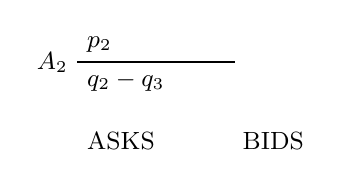
\begin{tikzpicture}
\node [right] at (0,0) {\small ASKS};
\node [left] at (3,0) {\small BIDS};
\draw [thick] (0,1) --(2,1);
\node [above right] at (0,1) {\small $p_2$};
\node [below right] at (0,1) {\small $q_2-q_3$};
\node [left] at (0,1) {\small $A_2$};
\end{tikzpicture}
&
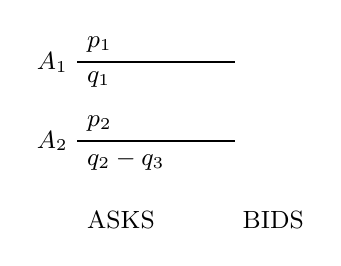
\begin{tikzpicture}
\node [right] at (0,0) {\small ASKS};
\node [left] at (3,0) {\small BIDS};
\draw [thick] (0,1) --(2,1);
\node [above right] at (0,1) {\small $p_2$};
\node [below right] at (0,1) {\small $q_2-q_3$};
\node [left] at (0,1) {\small $A_2$};
\draw [thick] (0,2) --(2,2);
\node [above right] at (0,2) {\small $p_1$};
\node [below right] at (0,2) {\small $q_1$};
\node [left] at (0,2) {\small $A_1$};
\end{tikzpicture}
\\
Addition of $o_3$ & Addition of $o_2$ & Match between $o_2$ and $o_3$ & Addition of $o_1
\end{tabular}
\end{center}~

\end{document}